\documentclass[11pt]{article}

\usepackage[margin=1.5in]{geometry}

\usepackage{fancyhdr}
\pagestyle{fancy}
\newcommand\course{ASTR 101}
\newcommand\hwnumber{5}
\newcommand\duedate{November 17, 2020}

\lhead{Oliver Tonnesen\\V00885732}
\chead{\textbf{\Large Lab \hwnumber{} Report}}
\rhead{\course\\\duedate}

\usepackage[
	backend=biber,
	url=true
]{biblatex}
\addbibresource{lab5.bib}
\usepackage{enumitem}
\usepackage{float}
\usepackage{graphicx}
\usepackage{url}
\usepackage{pgfplots}
\pgfplotsset{width=10cm,compat=1.9}

\usepackage{multirow}

\usepackage{amsmath,amsfonts,amssymb}


\begin{document}
\section{Objective}
This lab exercise examines how Kepler used observations of orbits to come up with his three famous laws, and how they can be applied to predict various properties of planets' orbits.
This lab mainly comprises recreating the method used by Kepler to triangulate the positions of Mars and use them to determine its elliptical orbit.


\section{Introduction}
Kepler came up with his three laws of planetary motion based on the analysis of observations of Mars and other planets made by Tycho Brahe.

The observations used in this lab to recreate Kepler's analysis consist of a heliocentric longitude of Earth and a corresponding geocentric longitude of Mars for a set of six positions in Mars' orbit.
Any two observations of Mars at the same position in its orbit taken from different positions in Earth's orbit can be used to triangulate Mars' distance from us.
We can use this technique with a set of several positions in Mars' orbit to estimate its entire orbit.
This is especially straightforward since we know Mars' orbit should be in the shape of an ellipse.


\section{Procedure}
We begin by drawing a circle with a radius of 5 cm to represent Earth's orbit, which is very nearly circular.
For each position in Mars' orbit, we are given two sets of observations (a heliocentric longitude of Earth and a geocentric longitude of Mars).
We measure the angle of the heliocentric longitude of Earth and draw a line from the centre of the circle intersecting it.
From here, we measure the geocentric longitude of Mars and draw a line in that direction.
We do this for both observations, and wherever the two lines intersect is where Mars is in its orbit for that position.

Once we've done this for all six positions, we fit an ellipse to the six points, and take this to be Mars' orbit.
We take the line connecting the two furthest of the positions to be the major axis of Mars' orbit.

The final product can be seen in Figure~\ref{fig:mars-orbit}.


\section{Observations, Tables, and Graphs}
\begin{table}[h]
\caption{Distance between the Sun and Mars at each observed position.}
\begin{center}
\begin{tabular}{| c | c | c |}
	\hline
	Position & Distance (cm) & Distance (AU)\\ \hline
	A & 7.0 & 1.4 \\ \hline
	B & 6.9 & 1.4 \\ \hline
	C & 7.8 & 1.6 \\ \hline
	D & 8.7  & 1.7 \\ \hline
	E & 8.8 & 1.8 \\ \hline
	F & 6.7 & 1.3 \\
	\hline
\end{tabular}
\end{center}
\label{table:distances}
\end{table}

\begin{figure}[H]
\caption{Mars' estimated orbit (green ellipse) based on the triangulation of six positions in its orbit.}
\begin{center}
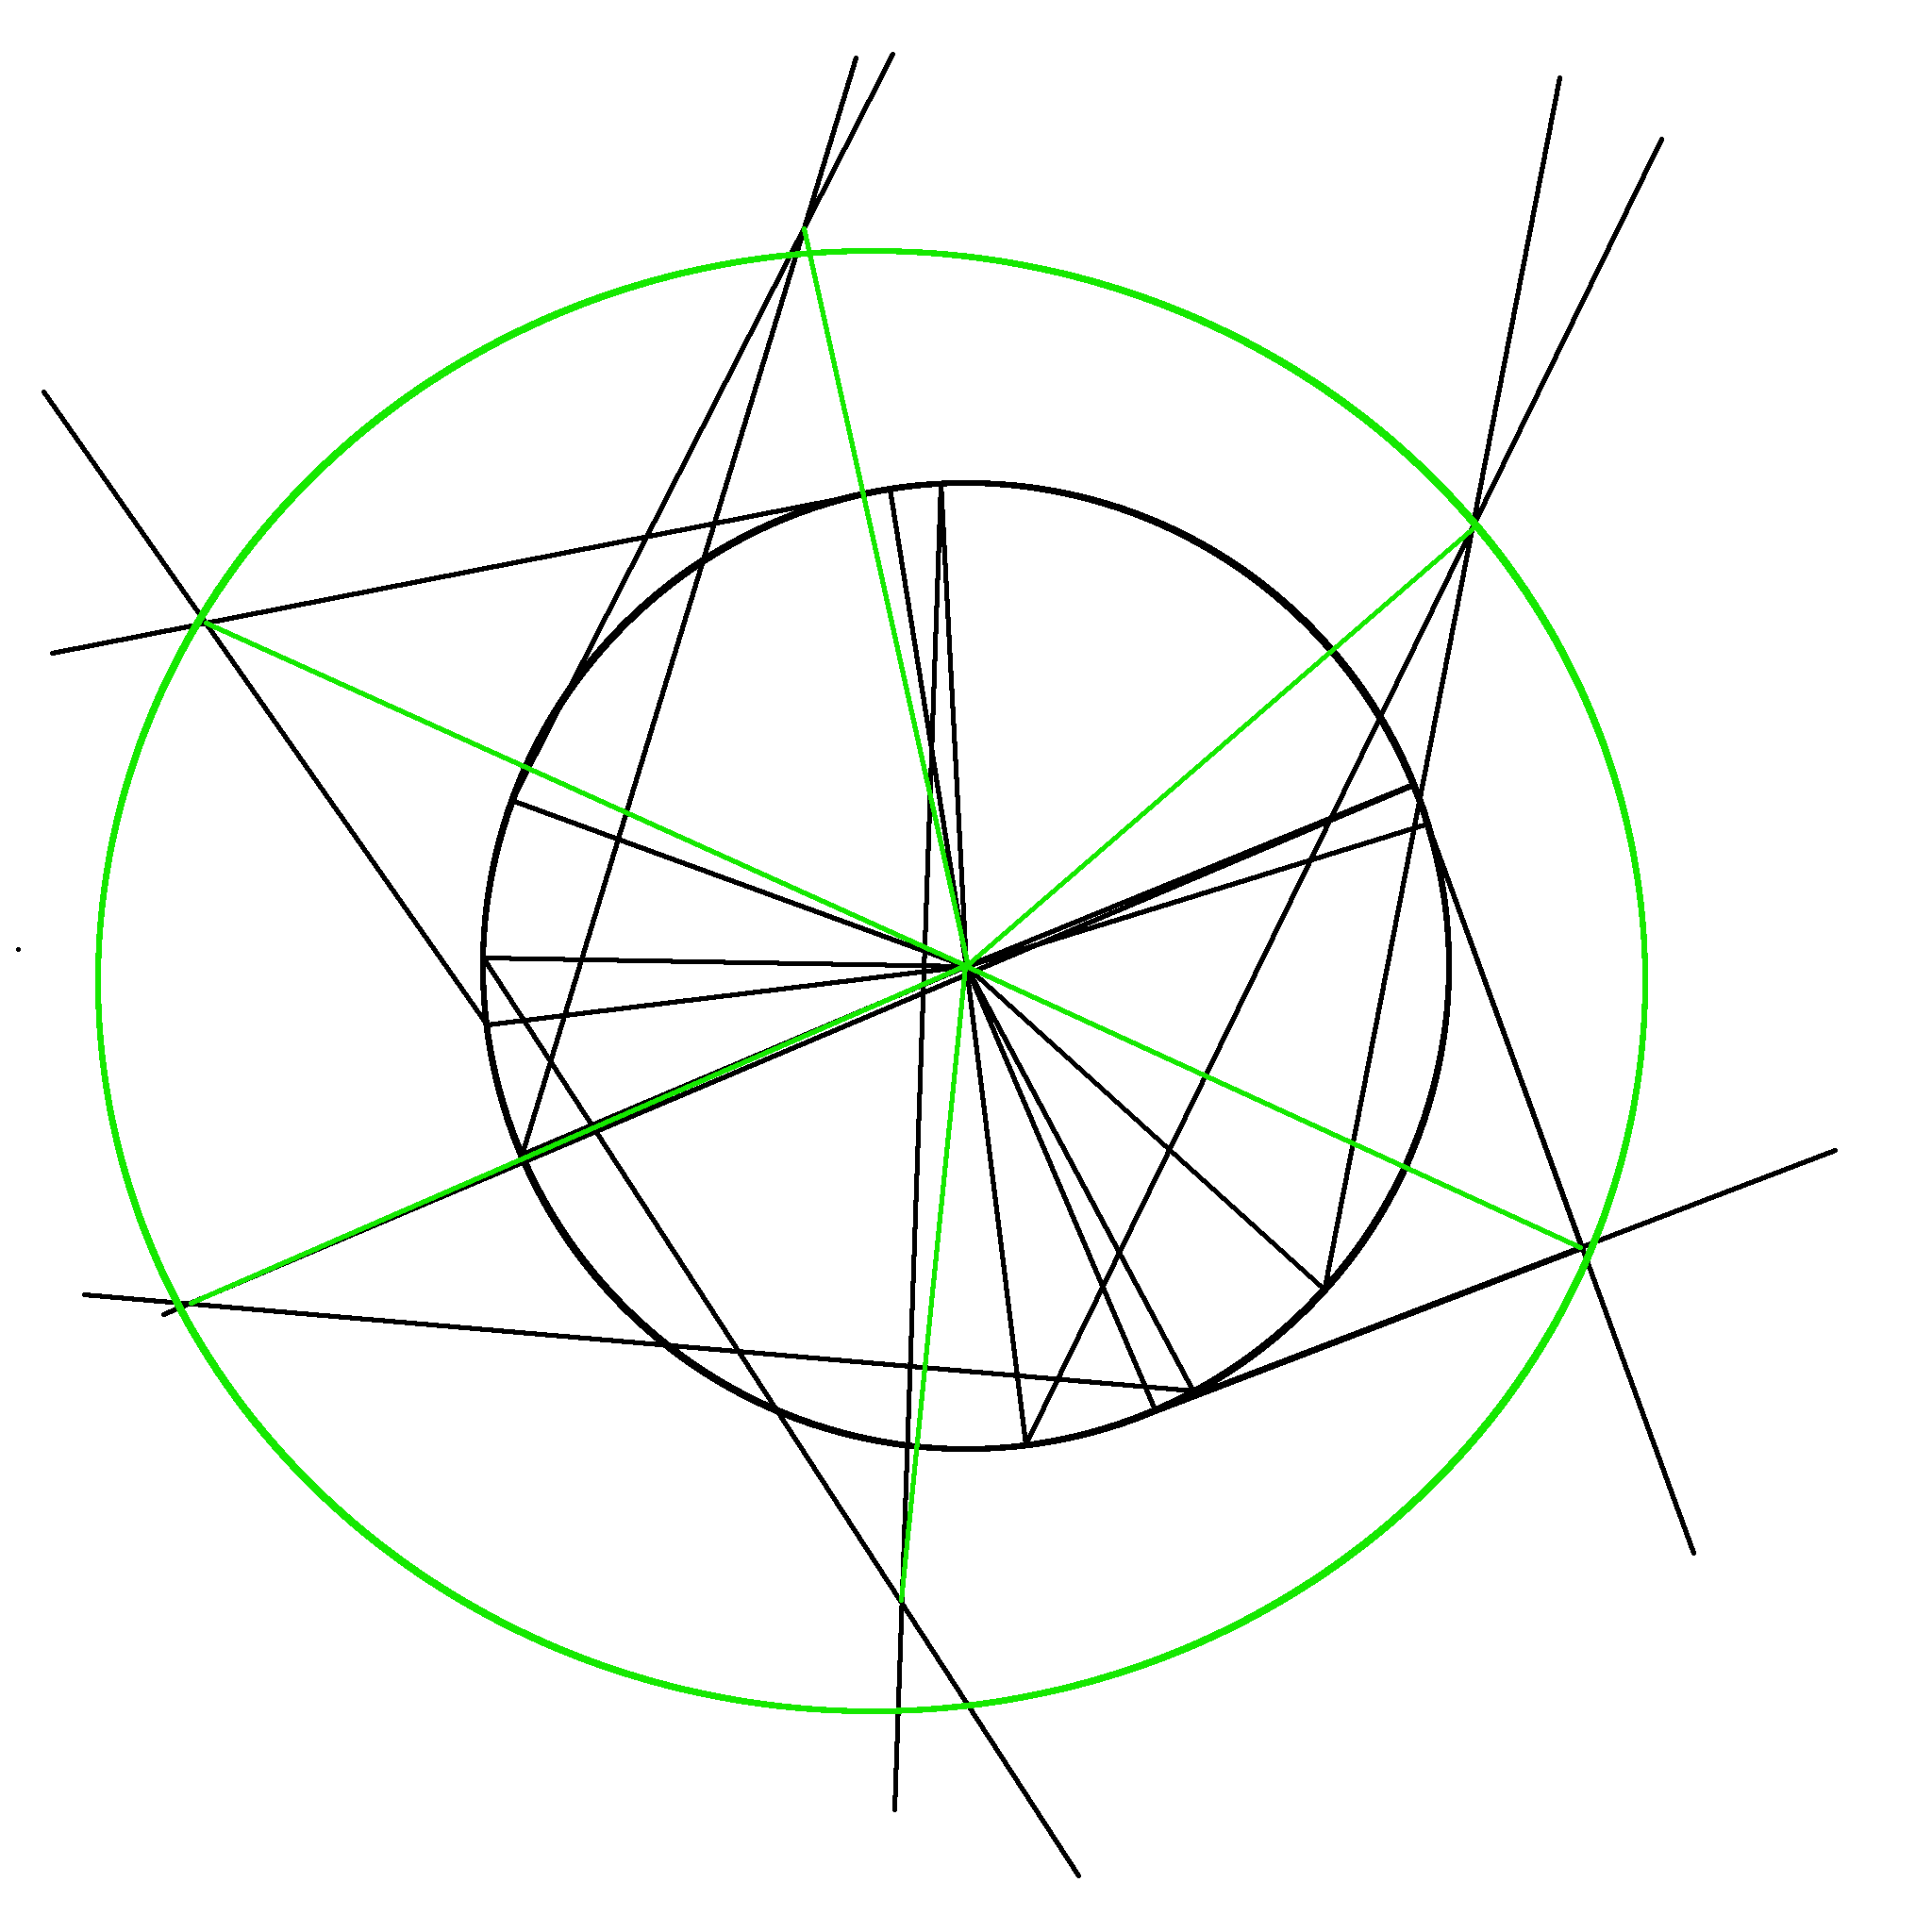
\includegraphics[scale=0.15]{figures/mars-orbit.png}
\end{center}
\label{fig:mars-orbit}
\end{figure}


\section{Calculations}
\subsection*{Centimetres to Astronomical Units}
We drew the Earth's orbit to be circular with radius 5 cm, so the conversion from cm to AU is simply $\frac{1\;\textrm{AU}}{5\;\textrm{cm}}$.
Below is a sample calculation of the distance between Earth's orbit and position A in AU:
\[7.0\;\textrm{cm} \cdot \frac{1.0\;\textrm{AU}}{5.0\;\textrm{cm}} = 1.4\;\textrm{AU}\]

\subsection*{Ratio of planet's period with $\frac{3}{2}$ power of its major axis length}
Mars' major axis length was measured to be 15.7 cm, giving us a length in AU of $15.7\;\textrm{cm} \cdot \frac{1.0\;\textrm{AU}}{5.0\;\textrm{cm}} = 3.1\;\textrm{AU}$.
Using the formulation of Kepler's third law given in \cite{UniPhys}, we calculate the ratio between the period and the $\frac{3}{2}$ power of the major axis length for Earth:
\[\frac{365\;\textrm{days}}{(1\;\textrm{AU})^{1.5}} = 365\]
and for Mars:
\[\frac{687\;\textrm{days}}{(1.5\;\textrm{AU})^{1.5}} = 374.\]


\section{Answers}
\begin{enumerate}[label={\textbf{\emph{(\arabic*)}}}]
	\item % 1
\cite{UniPhys} gives the following formulations of Kepler's three laws of planetary motion:
\begin{enumerate}[label=\arabic*.]
	\item % 1
Each planet moves in an elliptical orbit, with the sun at one focus of the ellipse.

	\item % 2
A line from the sun to a given planet sweeps out equal areas in equal times.

	\item % 3
The periods of the planets are proportional to the $\frac{3}{2}$ powers of the major axis lengths of their orbits.

\end{enumerate}

	\item % 2
The distance from the Sun to each of the six positions of Mars can be found in Table~\ref{table:distances}.
The average of these distances is 1.5 AU.

	\item % 3
We measured the major axis to of our ellipse to be 15.7 cm (the distance between points A and D), so our semi-major axis is 7.85 cm.
We measured the focal length of our ellipse to be 0.82 cm.
The eccentricity of our ellipse is thus $\frac{0.82\;\textrm{cm}}{7.85\;\textrm{cm}} \approx 0.10$.

	\item % 4
We measured the perihelion distance to be 7.0 cm and the aphelion distance to be 8.7 cm

	\item % 5
We know that the Martian year is nearly twice as long as a year on Earth (687 Earth days, or around 1.9 Earth years), so Mars is in opposition around twice per Martian year.
So every year, Mars is on approximately the opposite side of its elliptical orbit.
Note that if Mars' year was \emph{exactly} twice that of Earth's, then it would approach closer than average exactly half the time, since Mars would be in opposition in exactly two spots, alternating each Earth-year.
Since Mars' year is \emph{not} exactly twice that of Earth's, the two points in Mars' orbit at which opposition occurs shift slightly with each opposition.
That said, any pair of consecutive oppositions of Mars will still occur on roughly opposite sides of Mars' orbit, and so Mars will approach Earth closer than average roughly half the time.

	\item % 6
Since we assume that the Earth's orbit is circular, Mars is closest in opposition when it is at its perihelion, and is farthest when it is at its aphelion.
Based on our drawing, it appears Earth orbits closest to Mars' perihelion in October, and orbits closest to Mars' aphelion in March.

	\item % 7
The ratio of Earth's period with the $\frac{3}{2}$ power of the major-axis length of its orbit is 365, and Mars' is 374.
These values are quite close, and certainly reinforce Kepler's prediction that this ratio should be the same for any planet.

\end{enumerate}


\section{Discussion}
\subsection*{Discrepancies in calculated values}
According to \cite{nasa-mars}, Mars' average distance from the Sun is about 1.53 AU.
This is -- up to the precision of our measurement tool, one tenth of a centimetre -- exactly what we measured Mars' average distance to be.

According to \cite{nasa-mars2}, Mars' major axis has length approximately 3.047 AU.
Our calculated length for Mars' major axis was 3.1 AU.
This is reasonably close, and well within a margin for human error in the measurements we used in this calculation.

According to \cite{nasa-mars2}, Mars' orbital eccentricity is 0.0935.
This is close to our estimate of 0.10, but relatively less accurate than our estimations for Mars' average distance from the Sun and major axis length.
A likely reason for this discrepancy is the fact that this calculation required two measurements: one to the centre of Mars' major axis, and one from this centre point to the focus centred on the Sun.
Error from these two consecutive measurements likely compounded against us, resulting in a less accurate prediction.


\subsection*{Effects of Earth's assumed circular orbit}
In this lab, we assumed for simplicity that Earth's orbit has eccentricity 0, while in reality it has eccentricity 0.0167.
The main area in which this affects our lab is in our prediction of when Earth and Mars are closest in opposition.
It is the case that the major axes of Earth's and Mars' orbits are not parallel, and so we cannot simply say that Earth and Mars are closest in opposition when Earth lies on the line intersecting the Sun and Mars' perihelion.
For example, it could be the case that Earth and Mars are closer in opposition when Earth is at its perihelion and Mars is slightly past its perihelion.  
Since the eccentricity of Earth's orbit is in fact quite close to 0, it is unlikely that this is a reason for our estimation to be very far from reality.

The other way in which our results may be affected by this simplification is in the triangulation of our six observed positions of Mars.
Since our initial circle does not reflect Earth's orbit in reality, the points at which our lines intersect Earth's orbit might be slightly off, meaning our estimated positions of Mars are also slightly off.


\subsection*{Mars in opposition}
According to \cite{nasa-mars3}, the Mars' opposition in 2003 was the closest in nearly 60 000 years, and similar close oppositions occur every 15 to 17 years.
This year a close opposition occurred on October 13, the same month we predicted close approaches would occur in.
Next year a far opposition will occur, where Mars will be close to its aphelion.


\section{Conclusion}
In this lab exercise, we learned about how Kepler predicted his three laws based on limited observations.
We recreated his model of Mars' orbit to see how he used his observations to triangulate the positions of Mars and determine its orbit, and how he used this model orbit to make claims about the nature of the orbit of all planets, including Earth.


\printbibliography


\end{document}
